\documentclass[10pt,a4paper]{article}

\usepackage[a4paper,left=0.68in,right=0.68in,top=0.62in,bottom=0.60in,headheight=13pt]{geometry}
\usepackage[T1]{fontenc}
\usepackage{lmodern}
\usepackage{microtype}
\usepackage{amsmath,amssymb,mathtools}
\usepackage{booktabs}
\usepackage{enumitem}
\usepackage{xcolor}
\usepackage{tikz}
\usetikzlibrary{arrows.meta,positioning,calc,fit,shapes.geometric}
\usepackage{caption}
\usepackage{fancyhdr}
\usepackage{titlesec}
\usepackage[hidelinks]{hyperref}
\usepackage{multicol}

\pagestyle{fancy}
\fancyhf{}
\lhead{Department of Computer Science and Engineering}
\rhead{Context Compression for Long-Horizon LLM Agents}
\cfoot{\thepage}

\titleformat{\section}{\large\bfseries}{\thesection.}{0.4em}{}
\titleformat{\subsection}{\normalsize\bfseries}{\thesubsection}{0.35em}{}
\setlist[itemize]{leftmargin=1.35em,itemsep=1pt,topsep=1pt}
\setlist[enumerate]{leftmargin=1.6em,itemsep=1pt,topsep=1pt}
\setlength{\parindent}{0pt}
\setlength{\parskip}{2pt}
\captionsetup{font=small,labelfont=bf}
\setlength{\abovedisplayskip}{5pt}
\setlength{\belowdisplayskip}{5pt}

\begin{document}

% ============================================================
% TITLE PAGE
% ============================================================
\thispagestyle{empty}

\begin{center}

\vspace*{0.45cm}

{\Large\bfseries
INDIAN INSTITUTE OF INFORMATION TECHNOLOGY\\
DESIGN AND MANUFACTURING KURNOOL
}

\vspace{0.25cm}

{\normalsize
Department of Computer Science and Engineering
}

\vspace{1.25cm}

{\Large\bfseries MID-SEMESTER PROJECT REPORT}

\vspace{0.6cm}

\rule{0.78\textwidth}{0.6pt}

\vspace{0.65cm}

% TODO: confirm final project title
{\LARGE\bfseries
Composing Context Compression\\
for Long-Horizon LLM Agents
}

\vspace{0.35cm}

{\large
\textit{Controlled Composition and Critical-Fact Retention\\
on top of ACON}
}

\vspace{0.65cm}

\rule{0.78\textwidth}{0.6pt}

\vspace{0.8cm}

{\normalsize
A report submitted in partial fulfilment of the requirements\\
for the award of the degree of
}

\vspace{0.35cm}

{\Large\bfseries
Bachelor of Technology
}

\vspace{0.15cm}

{\large
Computer Science and Engineering
}

\vfill

{\large\bfseries
Submitted by
}

\vspace{0.35cm}

\renewcommand{\arraystretch}{1.35}

\begin{tabular}{c l}
\textbf{[ROLL NO. 1]} & \textbf{[STUDENT NAME 1]}\\
\textbf{[ROLL NO. 2]} & \textbf{[STUDENT NAME 2]}\\
\textbf{[ROLL NO. 3]} & \textbf{[STUDENT NAME 3]}
\end{tabular}

\vspace{1.0cm}

{\large\bfseries
Project Supervisor
}

\vspace{0.3cm}

{\large
[SUPERVISOR NAME]
}

\vfill

\rule{0.55\textwidth}{0.4pt}

\vspace{0.35cm}

{\normalsize
Department of Computer Science and Engineering\\
Indian Institute of Information Technology Design and Manufacturing Kurnool\\
Kurnool, Andhra Pradesh -- 518008
}

\vspace{0.35cm}

{\normalsize
September 2026
}

\end{center}

\newpage

% ============================================================
% 1. INTRODUCTION
% ============================================================
\section{Introduction}

LLM agents solve long-horizon tasks by alternating actions and observations
over tens of steps, and every tool output and intermediate thought is appended
to the prompt. The context therefore grows without bound. This causes two
problems: inference memory grows with the KV cache, and long, partly stale
contexts distract the model and degrade its decisions \cite{ACON}. Losing a
single file path or API token can derail an entire trajectory, so compression
must be aggressive and precise at the same time.

Existing methods compress one kind of context at a time: the interaction
history, the latest observation, or a document. Agents need several of these
stages at once, and it is not known how they interact. This project takes
ACON \cite{ACON} as the base method. We reproduce it and SAC \cite{SAC} on our
own hardware, and study how compression stages should be \emph{composed} and
\emph{evaluated}.

% ============================================================
% 2. LITERATURE REVIEW
% ============================================================
\section{Literature Review}

\textbf{Generative, prompt-level compression.} ACON \cite{ACON} uses an LLM to
rewrite the history once it exceeds a threshold $T_{\mathrm{hist}}$ and to
shorten observations longer than $T_{\mathrm{obs}}$. The compression guideline
is optimised in natural language: trajectories that succeed without
compression but fail with it are contrasted to produce feedback, and the
compressor is then distilled into smaller models. On AppWorld \cite{AppWorld}
with gpt-4.1, history compression reaches 56.5\% accuracy against 56.0\% with
no compression, and peak tokens drop by 26--54\% across three benchmarks.

\textbf{Soft, KV-level compression.} SAC \cite{SAC} selects anchor tokens from
the context, marks them with a learned embedding, and uses bidirectional
attention so that their key-value pairs absorb the whole context, without
autoencoding pretraining. On MRQA with Llama-3.2-1B at 15$\times$
compression, it reaches 54.95 in-domain F1, above EPL (51.52).

\textbf{Extractive, code-specific pruning.} SWE-Pruner \cite{SWEPruner} places
a 0.6B line-level classifier between a coding agent and its tools. The agent
writes a goal hint that conditions which lines of retrieved code are kept. On
SWE-Bench Verified it cuts tokens by 23--38\% while raising the resolve rate
by 1.2--1.4 points.

\textbf{Token pruning and RL-trained memory.} LLMLingua \cite{LLMLingua}
removes low-information tokens using a small language model. It is
task-agnostic, and in ACON's AppWorld comparison it reaches 39.3\% accuracy
for history compression. MEM1 \cite{MEM1} and MemAgent \cite{MemAgent} instead
train the agent with RL to maintain a bounded memory. MemAgent extrapolates
from an 8K window to 3.5M-token QA with under 10\% loss, but these methods
require updating the agent's weights.

\begin{table}[h]
\centering
\scriptsize
\renewcommand{\arraystretch}{1.12}
\setlength{\tabcolsep}{3pt}
\begin{tabular}{p{0.19\textwidth}cccccc}
\toprule
\textbf{Property} & \textbf{ACON} & \textbf{SAC} & \textbf{SWE-Pruner} &
\textbf{LLMLingua} & \textbf{MEM1/MemAgent} & \textbf{Proposed}\\
\midrule
Output form & Text & KV cache & Text lines & Text tokens & Text memory & Text\\
Agent weights frozen & Yes & Yes & Yes & Yes & No & Yes\\
History compression & Yes & No & No & Yes & Merged & Yes\\
Observation compression & Yes & No & Yes & Yes & Merged & Yes\\
Composition studied & Partly & No & No & No & No & \textbf{Yes}\\
Intrinsic quality metric & No & No & No & No & No & \textbf{Yes (CFR)}\\
\bottomrule
\end{tabular}
\caption{Comparison of context-compression families. ``Partly'': ACON reports a
combined setting in an appendix ablation only. ``Merged'': one memory holds both.}
\label{tab:lit}
\end{table}

% ============================================================
% 3. RESEARCH GAPS
% ============================================================
\section{Research Gaps}

\begin{enumerate}[label=(\alph*)]
\item \textbf{Token savings do not become time savings.} ACON's compressor
generates autoregressively, and rewriting the history invalidates the agent's
KV cache, forcing the compressed prefix to be recomputed. ACON's own
measurement on AppWorld (Qwen3-14B agent and compressor, one A100) gives a
median of 73.24\,s per task without compression, 87.68\,s with history
compression and 101.92\,s with observation compression \cite{ACON}.

\item \textbf{The combined setting is schedule-confounded.} History compression
fires when $|h_t|>T_{\mathrm{hist}}$. Once observations are compressed first,
$|h_t|$ grows more slowly, so history compression fires at different steps and
on already-pruned text. ACON's combined history+observation setting
(45.8\% accuracy, versus 56.5\% and 53.6\% for history and observation
compression alone \cite{ACON}) therefore changes two things at once and is not
a clean composition of two treatments.

\item \textbf{Compression quality is only measured indirectly.} ACON and SAC
judge a compressor solely by downstream success or F1/EM. Neither measures
whether the specific facts the agent will need survive compression, so a
failure cannot be attributed to information loss rather than to the agent.
\end{enumerate}

% ============================================================
% 4. PROBLEM STATEMENT
% ============================================================
\section{Problem Statement}

Given a long-horizon agent with frozen weights, a history compressor and an
observation compressor, determine how the two stages should be composed and
scheduled so that the token savings of each are retained without lowering task
success. The comparison between single-stage and composed settings must hold
the compression schedule fixed, and compression quality must be measured
directly, as the retention of task-critical state, rather than inferred only
from task success.

% ============================================================
% 5. PROPOSED SOLUTION
% ============================================================
\section{Proposed Solution}

We propose three changes to ACON's pipeline (Figure~\ref{fig:pipe}).

\textbf{1. Decoupled composition order.} The observation compressor still
produces a short $o'_t$ for the agent's immediate step, but the raw $o_t$ is
retained in a side buffer. When history compression fires, it summarises the
raw observations rather than the already-pruned ones, so information discarded
by the observation stage can still enter the history summary.

\textbf{2. Controlled compression schedule.} The trigger steps recorded in
the history-only run are replayed unchanged in the composed run, instead of
recomputing $|h_t|>T_{\mathrm{hist}}$ on pruned text. Single-stage and
composed conditions then differ only in the treatment, which removes the
confound of gap~(b).

\textbf{3. Critical-Fact Retention (CFR).} From each uncompressed trajectory
we extract state variables the agent later uses: access tokens, entity IDs,
file paths and numeric values. With $F$ the set of such facts present before a
compression call and $c$ the compressor output,
\[
\mathrm{CFR}=\frac{1}{|F|}\sum_{f\in F}\mathbf{1}\!\left[f \text{ appears verbatim in } c\right].
\]
CFR is an exact-match survival rate that can be computed per compression call
without rerunning the agent, and correlated with task success.

\begin{center}
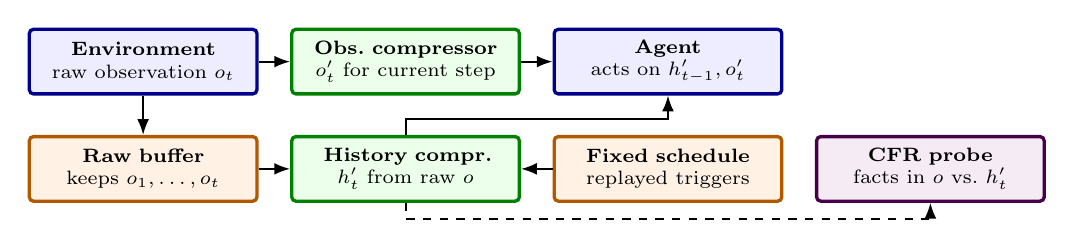
\begin{tikzpicture}[
  font=\scriptsize,
  bx/.style={draw, rounded corners=1.5pt, very thick, align=center,
    text width=2.75cm, minimum height=0.82cm, inner sep=2pt},
  arr/.style={-{Latex[length=2mm]}, line width=0.7pt},
  env/.style={bx, fill=blue!7, draw=blue!55!black},
  cmp/.style={bx, fill=green!8, draw=green!50!black},
  ctl/.style={bx, fill=orange!10, draw=orange!70!black},
  met/.style={bx, fill=violet!8, draw=violet!55!black}
]
\node[env] (o) {\textbf{Environment}\\raw observation $o_t$};
\node[cmp, right=4mm of o] (oc) {\textbf{Obs.\ compressor}\\$o'_t$ for current step};
\node[env, right=4mm of oc] (ag) {\textbf{Agent}\\acts on $h'_{t-1},o'_t$};
\node[ctl, below=5mm of o] (buf) {\textbf{Raw buffer}\\keeps $o_1,\dots,o_t$};
\node[cmp, right=4mm of buf] (hc) {\textbf{History compr.}\\$h'_t$ from raw $o$};
\node[ctl, right=4mm of hc] (sch) {\textbf{Fixed schedule}\\replayed triggers};
\node[met, right=4mm of sch] (cfr) {\textbf{CFR probe}\\facts in $o$ vs.\ $h'_t$};
\draw[arr] (o)--(oc);
\draw[arr] (oc)--(ag);
\draw[arr] (o)--(buf);
\draw[arr] (buf)--(hc);
\draw[arr] (sch)--(hc);
\draw[arr] (hc.north) -- ++(0,0.2) -| (ag.south);
\draw[arr, dashed] (hc.south) -- ++(0,-0.2) -| (cfr.south);
\end{tikzpicture}
\end{center}
\captionof{figure}{Proposed pipeline. The history compressor reads raw
observations from a side buffer (orange), fires on a schedule fixed across
conditions, and every call is scored by the CFR probe (violet).}
\label{fig:pipe}

% ============================================================
% 6. IMPLEMENTATION AND RESULTS
% ============================================================
\section{Implementation and Results}

\textbf{Setup.} All runs use one NVIDIA RTX 2000 Ada (16\,GB). For ACON,
models are served locally through Ollama: the agent is \texttt{qwen2.5:14b}
and the compressor \texttt{qwen2.5:7b}. We use the AppWorld
\texttt{train\_history\_tiny} split (38 tasks) with seed 42 and temperature 0.
For SAC, we use the authors' Llama-3.2-1B checkpoints on MRQA.

\textbf{ACON reproduction (preliminary).} Table~\ref{tab:acon} reports our
AppWorld runs. The fast runs use 8 tasks with at most 12 iterations. The full
history-compression run had completed 18 of 38 tasks at the time of writing,
so it is compared with the baseline on the same 18 tasks. On these, history
compression solved 9 tasks against 7 and used 24.5\% fewer agent input tokens.
The change is not uniform: it solved 5 tasks the baseline failed and failed 3
the baseline solved. On the 8-task fast runs, both compression settings
finished slightly sooner than the baseline, so the latency overhead ACON
reports (gap (a)) did not appear at this scale.

\begin{table}[h]
\centering
\scriptsize
\renewcommand{\arraystretch}{1.12}
\setlength{\tabcolsep}{4pt}
\begin{tabular}{p{0.34\textwidth}cccccc}
\toprule
\textbf{Run} & \textbf{Tasks} & \textbf{Max iter.} & \textbf{Solved} &
\textbf{Avg iter.} & \textbf{Agent input tok.} & \textbf{Wall clock (s)}\\
\midrule
Baseline, no compression & 8 & 12 & 1 & 11.00 & 269,935 & 953.9\\
History compression ($T_{\mathrm{hist}}=512$) & 8 & 12 & 2 & 10.75 & 232,749 & 882.8\\
Observation compression ($T_{\mathrm{obs}}=256$) & 8 & 12 & 1 & 11.00 & 261,422 & 873.6\\
\midrule
Baseline, full split & 38 & 30 & 12 (31.6\%) & 23.7 & 2,972,376 & 7312\\
\midrule
Baseline, matched subset & 18 & 30 & 7 & 22.22 & 1,283,906 & not logged\\
History compression, matched subset & 18 & 30 & 9 & 19.50 & 969,389 & not logged\\
\bottomrule
\end{tabular}
\caption{Preliminary ACON runs on AppWorld (\texttt{qwen2.5:14b} agent,
\texttt{qwen2.5:7b} compressor, seed 42). Wall-clock time is not logged for
the matched subset because the baseline's progress log is incomplete.}
\label{tab:acon}
\end{table}

These numbers carry three caveats. First, Ollama served both models with a
4096-token context, so long baseline prompts were truncated and part of any
gain may come from staying under this limit. Second, thresholds are 512/256
rather than the paper's 4096/1024, because the paper values rarely fire on
this split. Third, each setting was run with a single seed.

\textbf{SAC reproduction.} Evaluating the released checkpoints reproduces the
published macro-averaged MRQA scores to within 0.2 F1: at 15$\times$ we obtain
54.98 in-domain / 39.25 out-of-domain F1 (published 54.95 / 39.26), and at
5$\times$ 63.70 / 47.71 (published 63.63 / 47.72).

\textbf{SAC$\times$ACON pilot (preliminary).} We trained two ACON-inspired
variants of SAC for 5,000 steps at 15$\times$ (single seed, evaluated on
6,786 examples) against a matched SAC control (51.37 / 38.62 F1).
Failure-gated distillation, which distils from the full-context model only
where compression fails, gave $-0.23$ in-domain F1 (95\% CI
$[-0.95,+0.47]$), i.e.\ no effect. Task-guided anchors combined with
failure-gated distillation reached 60.03 / 44.71 F1, a gain of $+8.66$
$[+7.66,+9.60]$ in-domain. That variant sees the question during compression,
so it is not directly comparable to question-agnostic SAC, and task-guided
anchors alone have not yet been run.

% ============================================================
% 7. CONCLUSION
% ============================================================
\section{Conclusion}

We have reproduced SAC's published results and set up a local ACON pipeline
on AppWorld. On the 18 tasks run so far, history compression solves more
tasks with 24.5\% fewer agent input tokens. We identified three gaps in how
context compressors are composed and evaluated: latency, schedule confounding
and the lack of an intrinsic quality metric. Next, we will complete the
38-task history and observation runs and add runs at the paper thresholds.
We will then implement the raw-observation buffer, the fixed schedule and the
CFR metric, and evaluate the composed pipeline across multiple seeds.

\begin{thebibliography}{99}

\bibitem{ACON}
M. Kang, W.-N. Chen, D. Han, H. A. Inan, L. Wutschitz, Y. Chen, R. Sim, and
S. Rajmohan,
``ACON: Optimizing Context Compression for Long-horizon LLM Agents,''
in \emph{Proc. 43rd Int. Conf. Machine Learning (ICML)}, PMLR 306, 2026.

\bibitem{SAC}
X. Liu, R. Zhao, P. Huang, X. Liu, J. Xiao, C. Xiao, T. Xiao, S. Gao, Z. Yu,
and J. Zhu,
``Autoencoding-Free Context Compression for LLMs via Contextual Semantic
Anchors,''
in \emph{Int. Conf. Learning Representations (ICLR)}, 2026.

\bibitem{SWEPruner}
Y. Wang, Y. Shi, M. Yang, R. Zhang, S. He, H. Lian, Y. Chen, S. Ye, K. Cai,
and X. Gu,
``SWE-Pruner: Self-Adaptive Context Pruning for Coding Agents,''
arXiv:2601.16746, 2026.

\bibitem{LLMLingua}
H. Jiang, Q. Wu, C.-Y. Lin, Y. Yang, and L. Qiu,
``LLMLingua: Compressing Prompts for Accelerated Inference of Large Language
Models,''
in \emph{Proc. EMNLP}, pp. 13358--13376, 2023.

\bibitem{MEM1}
Z. Zhou, A. Qu, Z. Wu, S. Kim, A. Prakash, D. Rus, J. Zhao, B. K. H. Low, and
P. P. Liang,
``MEM1: Learning to Synergize Memory and Reasoning for Efficient Long-Horizon
Agents,''
arXiv:2506.15841, 2025.

\bibitem{MemAgent}
H. Yu, T. Chen, J. Feng, J. Chen, W. Dai, Q. Yu, Y.-Q. Zhang, W.-Y. Ma, J. Liu,
M. Wang, and H. Zhou,
``MemAgent: Reshaping Long-Context LLM with Multi-Conv RL-based Memory Agent,''
in \emph{Int. Conf. Learning Representations (ICLR)}, 2026.

\bibitem{AppWorld}
H. Trivedi, T. Khot, M. Hartmann, R. Manku, V. Dong, E. Li, S. Gupta,
A. Sabharwal, and N. Balasubramanian,
``AppWorld: A Controllable World of Apps and People for Benchmarking
Interactive Coding Agents,''
in \emph{Proc. ACL}, pp. 16022--16076, 2024.

\end{thebibliography}

\end{document}
